\section{Results}
\label{sect:results}

% |-----------------------------|
% | Comparison to observations. |
% |-----------------------------|
\subsection{Comparison to observations}
\label{sect:observations}

\begin{figure}
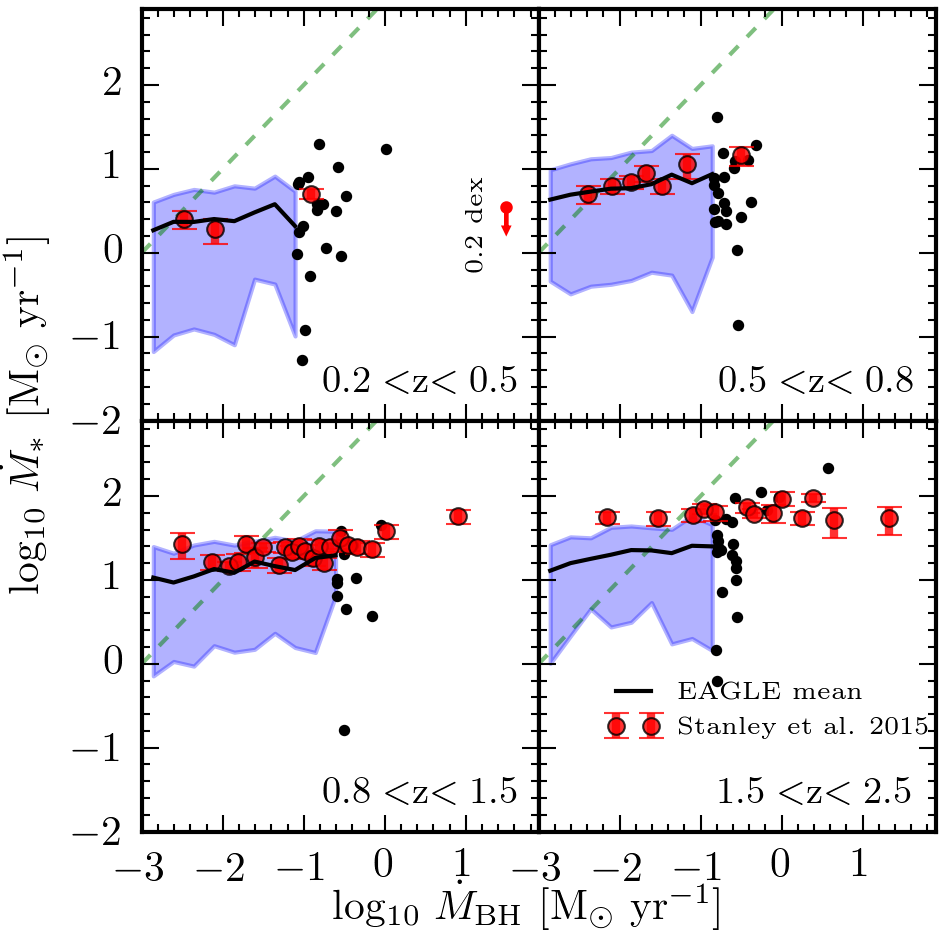
\includegraphics[width=\columnwidth]{plots/Stanley2015}

\caption{\SFR--\BHAR (SFR--BHAR) relation for four continuous redshift ranges
from $0.2 < z < 2.5$. BHARs are instantaneous and SFRs are the time-averaged
rate over the 100~Myr preceding the BH event. The \textit{mean} SFR as a
function of BHAR for central galaxies is shown as a black line, with the
corresponding blue shaded region indicating the 10-90$^{\mathrm{th}}$
percentile range. Bins containing fewer than 10 objects have their galaxies
represented individually as black solid circles.  The linear relation
\BHAR/\SFR = $10^{-3}$ is shown as a dashed green line and the data of
\citet{Stanley2015} is represented as red circles.  Fits to the \eagle mean
relations are tabulated in \cref{table:slopes}. The magnitude of the SFR
recalibration applied to the data for all redshifts is indicated by a red arrow
in the upper left panel (see \cref{sect:sfr_calibration}). For each redshift
range we find mean trends that are considerably flatter than a linear relation
($\gamma_{\mathrm{S15}} \ll 1$ in \cref{eq:slope4}).}

\label{fig:stanley2015}
\end{figure}

\begin{figure}
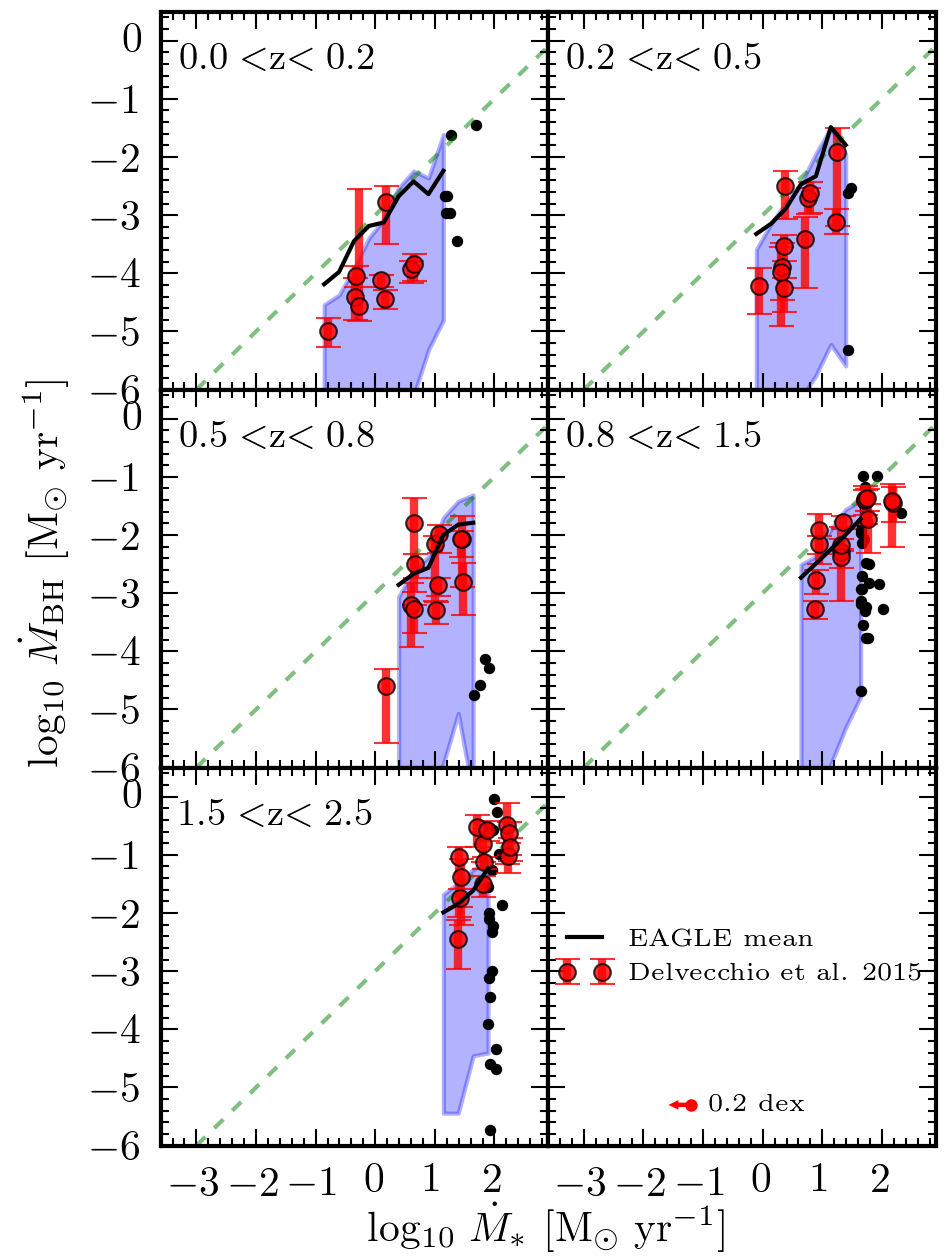
\includegraphics[width=\columnwidth]{plots/Delvecchio2015}

\caption{\BHAR--\SFR (BHAR--SFR) relation for five continuous redshift ranges
from $0.0 < z < 2.5$. BHARs are instantaneous and SFRs are the time-averaged
rate over the 100~Myr preceding the BH event. The \textit{mean} BHAR as a
function of SFR for central galaxies is shown as a black line, with the
corresponding blue shaded region indicating the 10-90$^{\mathrm{th}}$
percentile range. Bins containing fewer than 10 objects have their galaxies
represented individually as black solid circles.  The linear relation
\BHAR/\SFR = $10^{-3}$ is shown as a dashed green line and the data of
\citet{Delvecchio2015} is represented as red circles. Fits to the \eagle mean
relations are tabulated in \cref{table:slopes}. The magnitude of the SFR
recalibration applied to the data for all redshifts is indicated by a red arrow
in the lower right panel (see \cref{sect:sfr_calibration}). For each redshift
range we find gradients of the mean trend close to unity ($1 /
\gamma_{\mathrm{D15}} \approx 1$), in good agreement with a linear relation.}

\label{fig:delvecchio2015}
\end{figure}

\begin{table*}

\caption{Slope ($\gamma$) and intercept ($\delta$) of various relations
satisfying \cref{eq:slope4}. S15 denotes the study of \citet{Stanley2015} and
D15 denotes the study of \citet{Delvecchio2015}.  Columns 2 and 3 are the
fitted values of the \eagle mean relations investigated in
\cref{fig:stanley2015,fig:delvecchio2015}. Annotated with a * in columns 6 and
7 are the \eagle \emph{median} fits to the same datasets. Fits to the mean
relation of the 100~Myr time-averaged growth rates from \cref{sect:time_av} for
the same datasets are shown in columns 4 and 5. Errors on the individual
mean/median \eagle data points are taken from bootstrap re-sampling. Quoted
fits and their associated errors were computed using the Python module
\sc{lmfit}.}

\begin{tabular}{crrrrrrr} \hline
$z$ &
$\gamma_{\mathrm{S15}}$  &
log$_{10} \delta_{\mathrm{S15}}$  &
$\gamma_{\mathrm{S15}} \langle \mathrm{100 Myr} \rangle$ &
log$_{10} \delta_{\mathrm{S15}} \langle \mathrm{100 Myr} \rangle$ &
$\gamma_{\mathrm{S15}}$*  &
log$_{10} \delta_{\mathrm{S15}}$* \\
\hline\hline
0.20 < $z$ < 0.50 & $0.13 \pm 0.04$ & $0.67 \pm 0.09$ & $0.31 \pm 0.05$ & $1.18 \pm 0.14$ & $0.14 \pm 0.02$ & $0.46 \pm 0.05$ \\
0.50 < $z$ < 0.80 & $0.15 \pm 0.02$ & $1.07 \pm 0.04$ & $0.26 \pm 0.01$ & $1.36 \pm 0.04$ & $0.12 \pm 0.03$ & $0.83 \pm 0.07$ \\
0.80 < $z$ < 1.50 & $0.12 \pm 0.03$ & $1.32 \pm 0.06$ & $0.27 \pm 0.02$ & $1.63 \pm 0.04$ & $0.14 \pm 0.03$ & $1.23 \pm 0.07$ \\
1.50 < $z$ < 2.50 & $0.16 \pm 0.02$ & $1.60 \pm 0.05$ & $0.24 \pm 0.02$ & $1.72 \pm 0.05$ & $0.16 \pm 0.02$ & $1.51 \pm 0.05$ \\
\hline
$z$ & $1 / \gamma_{\mathrm{D15}}$  &
-$\frac{\mathrm{log}_{10} \delta_{\mathrm{D15}}}{\gamma_{\mathrm{D15}}}$ &
$1 / \gamma_{\mathrm{D15}} \langle \mathrm{100 Myr} \rangle$ &
log$_{10} \delta_{\mathrm{D15}} \langle \mathrm{100 Myr} \rangle$ &
$1 / \gamma_{\mathrm{D15}}$*  &
-$\frac{\mathrm{log}_{10} \delta_{\mathrm{D15}}}{\gamma_{\mathrm{D15}}}$* \\
\hline\hline
0.01 < $z$ < 0.25 & $1.07 \pm 0.10$  & $-3.21 \pm 0.05$ & $1.06 \pm 0.06$ & $-3.29 \pm 0.04$ & $2.68 \pm 0.14$ & $-5.52 \pm 0.07$ \\
0.25 < $z$ < 0.50 & $1.13 \pm 0.11$  & $-3.30 \pm 0.05$ & $0.94 \pm 0.04$ & $-3.07 \pm 0.02$ & $2.28 \pm 0.20$ & $-5.61 \pm 0.10$ \\
0.50 < $z$ < 0.80 & $1.06 \pm 0.19$  & $-3.35 \pm 0.17$ & $1.10 \pm 0.03$ & $-3.23 \pm 0.02$ & $2.21 \pm 0.33$ & $-5.99 \pm 0.29$ \\
0.80 < $z$ < 1.50 & $1.00 \pm 0.01$  & $-3.39 \pm 0.15$ & $1.27 \pm 0.03$ & $-3.44 \pm 0.03$ & $2.48 \pm 0.21$ & $-6.53 \pm 0.23$ \\
1.50 < $z$ < 2.50 & $0.96 \pm 0.16$  & $-3.17 \pm 0.24$ & $1.37 \pm 0.04$ & $-3.60 \pm 0.05$ & $1.61 \pm 0.26$ & $-5.18 \pm 0.39$ \\
\hline
\end{tabular}
\label{table:slopes}
\end{table*}

We begin by comparing the predicted relationship between galaxy and BH growth
rates to two recent observational studies using different selection criteria.
Firstly, we explore the \av{SFR} versus BHAR relation for the \textit{AGN
selected} sample presented by \citet{Stanley2015}.  Secondly, we explore the
\av{BHAR} versus SFR relation for the \textit{SFR selected} sample presented by
\citet{Delvecchio2015}. Together they represent two of the largest sample sizes
of their respective selection techniques, spanning multiple epochs. Large
sample sizes such as these are key in overcoming the uncertainties inherent to
low number statistics and in mitigating the potential redshift evolution biases
that could be misinterpreted as an underlying trend.

As mentioned in \cref{sect:individual_galaxies}, SFRs obtained via FIR tracers
most likely probe the recent star formation history of a galaxy, rather than an
instantaneous value. Therefore the comparative SFRs of \eagle galaxies used
in the analysis of \cref{fig:stanley2015,fig:delvecchio2015} are the
time-averaged rate over the 100~Myr preceding the instantaneous BHAR
measurement. However, when performing the equivalent analysis using the
instantaneous values of SFR at the time of the BHAR measurement we find no
difference in the result, attesting to the stability of star formation as a
process.   

\subsubsection{SFR as a function of BHAR for an AGN selected sample}

The study of \citet{Stanley2015} consists of $\approx 2000$ X-ray detected AGN
spanning over three orders of magnitude in luminosity ($10^{42} < $ \LXray$<
10^{45.5}$~erg~s$^{-1}$) for the redshift range $z=0.2 - 2.5$. To compare to
the data we convert their quoted bolometric AGN luminosities (derived from
X-ray luminosities) to BHARs via  

\begin{equation} 
\dot M_{\mathrm{BH}} = \frac{L_{\mathrm{AGN}}}{\epsilon_{r} c^{2}},
\label{eq:lagn}
\end{equation}

\noindent where $c$ is the speed of light and $\epsilon_{r}$ is the radiative
efficiency of the accretion disk, which is assumed to be 0.1
\citep{Shakura1973}. To emulate the sample selection of this study, we choose
\eagle galaxies based on a redshift independent detection limit of $\dot
M_{\mathrm{BH}} = 10^{-3}$~\Msol~yr$^{-1}$, corresponding to \LAGN$\approx
10^{43}$~erg~s$^{-1}$ according to \cref{eq:lagn} and is equivalent to \LXray
$\approx 10^{42}$~erg~s$^{-1}$ using the conversion methods outlined in Section
3.2 of \citet{Stanley2015}.

The results are presented in \cref{fig:stanley2015}, showing the
\textit{mean} SFR as a function of BHAR, represented by a solid black line. We
see that for each redshift range the gradient of the relation remains shallow
(note the same dynamic range is used for both axes), ranging in values $0.1
\leq \gamma_{\mathrm{S15}} \leq 0.2$ (see \cref{table:slopes}) and is in
striking agreement with the \dquotes{remarkably flat} relation reported by
\citet{Stanley2015}.  This is considerably flatter than one would predict for a
linear \M{BH}--\M{bulge,*} relation from a co-evolution of growth, which we
represent as a dashed green line\footnote{Using \cref{eq:slope3} with $\beta =
1000$ \citep{McConnellandMa2013}.} (see \cref{sect:motivation}). The dynamic
range of SFRs is modest, with a scatter of $\approx 1-1.5$~dex for all
redshifts.  The normalisations of \av{SFR} in the three lowest redshift ranges
($0.2 < z < 1.5$) are in good agreement with the observational estimates
(within $\approx 0.1$~dex).  However, the values in the highest redshift range
($1.5 < z < 2.5$) are systematically under predicted by $\approx 0.5$~dex over
and above the recalibration discussed in \cref{sect:sfr_calibration}. We note
that this highest bin is potentially subject to the largest systematic over
estimate ($\approx 0.4$~dex) due to the large fraction ($\approx 80$\%) of
undetected FIR sources (included as upper limits) in the observations
\citep[see][]{Stanley2015}.

\subsubsection{BHAR as a function of SFR for a SFR selected sample}

The study of \citet{Delvecchio2015} consists of $\approx 8600$ star-forming
galaxies detected out to $z=2.5$. The selection limits in SFR are redshift
dependent, corresponding to 0.2, 1.0, 3.0, 8.0 and 25.0 \Msolyr for the five
redshift ranges covered by this study from low to high respectively. We note
that the data points from \citet{Delvecchio2015} are segregated also in stellar
mass, however for simplicity we make no such distinction.

The comparison is shown in \cref{fig:delvecchio2015}, showing the \textit{mean}
BHAR as a function of SFR as the solid black line.  Again, \eagle shows a good
consistency with the observational measurements (shown in red), only over
predicting \av{BHAR} in the lowest redshift range ($0.0 < z < 0.5$).  However,
\citet{Delvecchio2015} mentions that the limited co-moving volume of this study
at low redshift could potentially exclude the most luminous sources.  The
behaviour of the \av{BHAR}--SFR relation is quite different from the
\av{SFR}--BHAR relation seen in \cref{fig:stanley2015}, adhering much closer to
a linear trend. We see, uniformly, gradients close to unity ($1.0 \leq 1 /
\gamma_{\mathrm{D15}} \leq 1.2$, see \cref{table:slopes}) in good agreement
with the linear \M{BH}--\M{bulge,*} relation expected for a co-evolution of
growth, shown as a dashed green line (note again the same dynamic range is used
for both axes).  An additional difference is the spread of values in the
minimisation axis (\BHAR for this figure). The distribution of SFRs in
\cref{fig:delvecchio2015} span a relatively narrow dynamic range, whereas here,
BHARs vary as much as $\approx 4$~dex in the $10-90^{\mathrm{th}}$ percentile
region.  In fact, the dynamic range of BHARs is so large that the small
fraction of galaxies whose values dominate the mean are able to pull it outside
this percentile range entirely in some places, suggesting the median to be a
more suitable statistic to measure this trend. 

Overall the agreement between \eagle and the observations is excellent,
particularly given that no information regarding this relation was considered
during the calibration procedure. The difference in behaviour found empirically
via alternate selection criteria is well reproduced by the simulation. We find,
consistent with the \citet{Hickox2014} model and findings by
\citet{Volonteri2015b}, that \av{SFR}--BHAR for an AGN selected sample exhibits
a relatively flat trend ($\gamma_{\mathrm{S15}} \approx 0.15$), whilst that of
\av{BHAR} with respect to SFR for a SFR selected sample is substantially
steeper and close to unity ($1 / \gamma_{\mathrm{D15}} \approx 1.1$). However,
within the paradigm of a linear \M{BH}--\M{bulge,*} relation created through
co-evolution of growth these results are both predicted to be linear (i.e,
$\gamma \approx 1$ for both, see \cref{sect:motivation}).  Therefore either the
underlying relationship itself is fundamentally non-linear, or a fuller
understanding of the two processes is required. In the next section we continue
to examine potential reasons as to the cause of this difference. 

\subsection{Understanding the BHAR-SFR relationship} \label{sect:understanding}

In this section we explore two potential reasons why the \av{SFR}--BHAR and
\av{BHAR}--SFR trends are not each consistent with a linear relationship. We
examine the hypothesis that (1) growth rates have an underlying linear
connection only on average, which is masked when the unstable growth rate is
observed instantaneously and (2) how selection biases due to the inability to
probe the complete SFR--BHAR plane may play a role.  

\subsubsection{A time-averaged SFR--BHAR connection}
\label{sect:time_av}

\citet{Hickox2014} suggested that an underlying correlation held between a
stable (galactic star formation) and unstable (BH accretion) process \textit{on
average} could be washed out if the unstable property is measured
instantaneously.  That is to say, if one could observe X-ray luminosities of
AGN sources over prolonged periods, the underlying relationship between the two
properties would begin to emerge.  Indeed, with a simple model that assumes SFR
and BHAR are connected on average with a linear scaling over a period of
100~Myr, \citet{Hickox2014} reproduce the empirical behaviours of both the
\av{SFR}--BHAR and \av{BHAR}--SFR relationships whilst retaining a scenario
consistent with a linear co-evolution between galaxies and their central BHs.
While it is not possible to test observationally due to the length of these
timescales, we are able to test this hypothesis using the simulation.

\cref{fig:avandinst} is similar to the upper left panel of
\cref{fig:stanley2015}. The region in blue, with the black solid line, shows
the original analysis of the \av{SFR}--BHAR relation for the redshift range
$0.2 < z < 0.5$ using instantaneous BHARs and SFRs that are time-averaged 100~Myr
before the BH event. Overlaid in red, with the mean represented by a dashed
line, is the same selection of galaxies (i.e, instantaneous \BHAR $>
10^{-3}$\Msolyr) with each growth rate now time-averaged over 100~Myr.
Interestingly, although the high BHARs shift systematically to lower values on
average\footnote{The shift ($\approx$0.5~dex) to lower values in BHAR when
averaging over 100~Myr arises due to the most luminous \squotes{detections}
commonly residing in peaks of the accretion rate history.}, both the dynamic
range and slope of the mean remain broadly consistent with their instantaneous
equivalents ($\gamma_{\mathrm{S15}} \rightarrow \gamma_{\mathrm{S15} \langle
100~\mathrm{Myr} \rangle} = 0.2 \rightarrow 0.3$, see \cref{table:slopes}).
This behaviour remains for each redshift range explored by \citet{Stanley2015}
(see \cref{table:slopes}).  An alternate approach is to select galaxies in
excess of \BHAR $= 10^{-3}$\Msolyr on average (rather than instantaneously as
done above) or indeed to prolong the averaging timescale to $> 100$~Myrs.
However in each case, and for all redshift intervals, the gradient values
remain well below unity ($0.30 < \gamma_{\mathrm{S15} \langle 100~\mathrm{Myr}
\rangle} < 0.55$).  This leads us to conclude that the average galaxy and BH
growth rates for an AGN selected sample do not harbour an underlying global
linear relationship. 

\begin{figure}
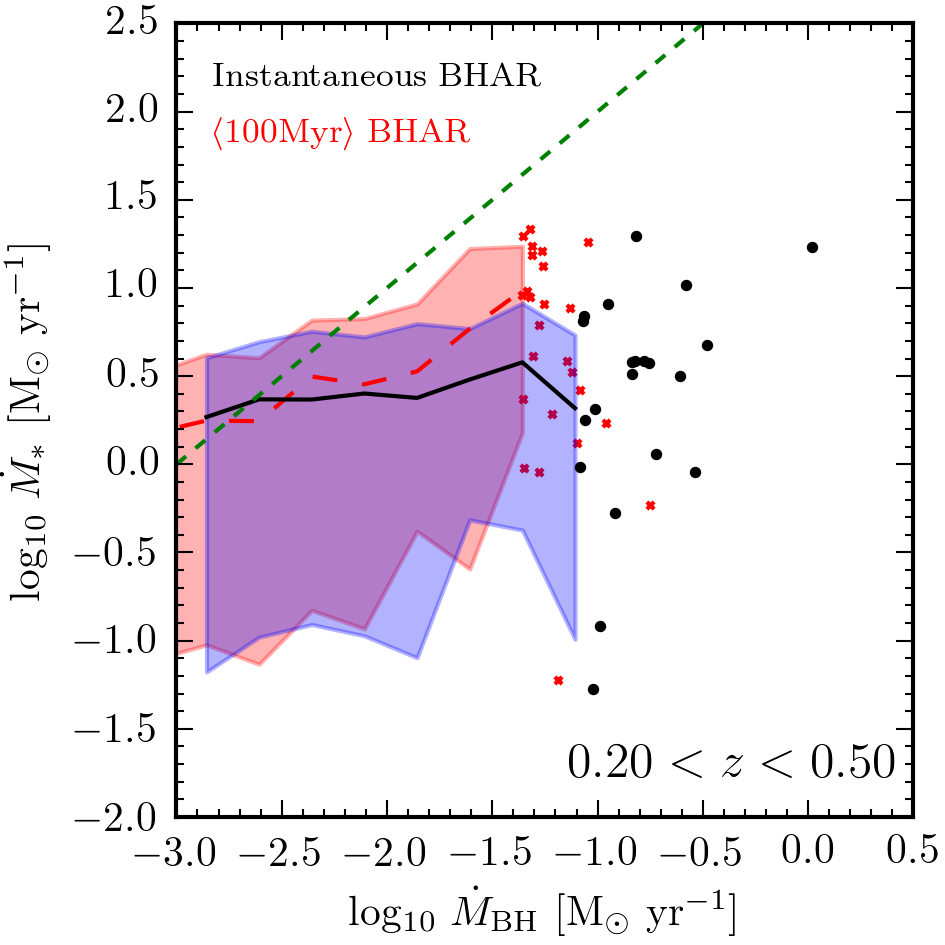
\includegraphics[width=\columnwidth]{plots/z1_AverageGrowthRates}

\caption{\textit{blue region}: A replica of the upper left panel in
\cref{fig:stanley2015} (see caption for description of contents). Here BHARs
are instantaneous and SFRs are the time-averaged rate over the 100~Myr
preceding the BH event. \textit{red region}: We repeat the analysis for the
same central galaxies satisfying the \citet{Stanley2015} selection criteria
(instantaneously, blue region), however now both SFR and BHAR are time-averaged
over the same 100~Myr period.  Fits to the time-averaged mean relations are
shown in \cref{table:slopes} (denoted with $\langle 100~ \mathrm{Myr}
\rangle$). We find that even when both growth rates are time-averaged over
100~Myr, an AGN selected sample does not revert to a linear relationship
between \SFR and \BHAR.}

\label{fig:avandinst} \end{figure}

% |---------------------|
% | The SFR-BHAR plane. |
% |---------------------|
\subsubsection{Sampling different regions of the entire SFR-BHAR plane}
\label{sect:sfr_vs_bhar_plane}

\begin{figure}
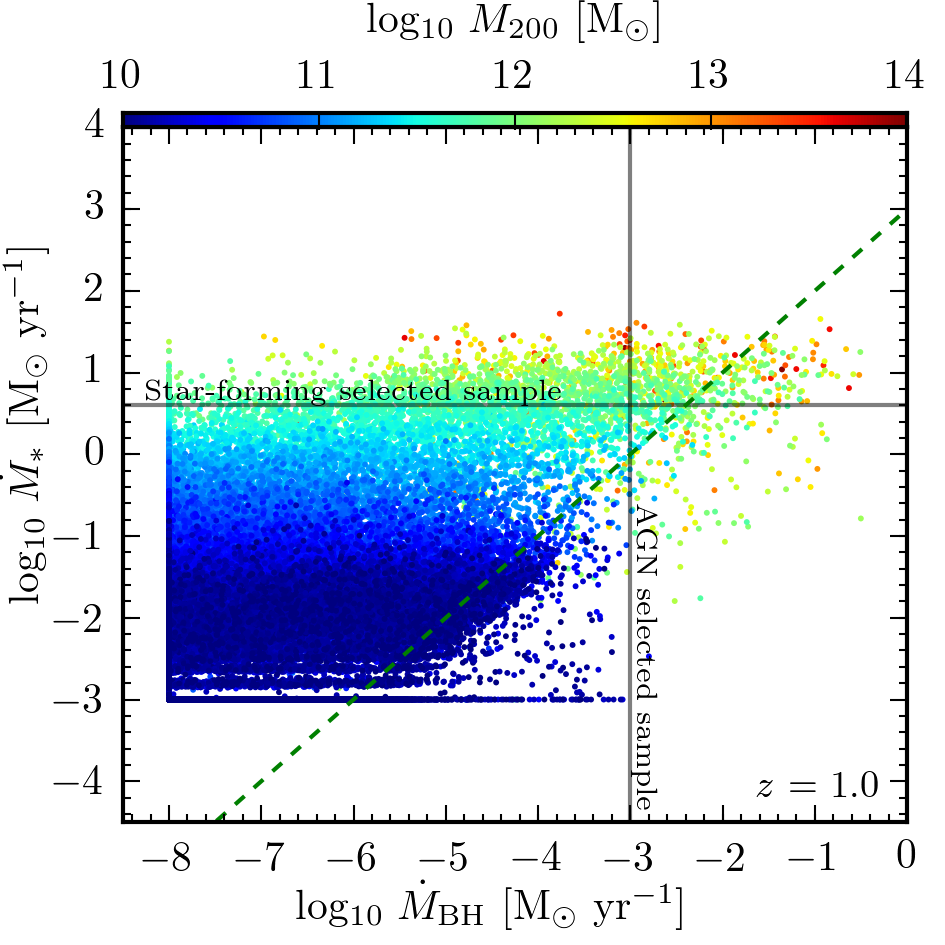
\includegraphics[width=\columnwidth]{plots/SFRvsBHAR_z1}

\caption{\SFR-\BHAR (SFR-BHAR) relation for central galaxies at $z=1$. Growth
rates are \textit{instantaneous} and coloured by the mass of the halo
(\M{200}). Values that are below $10^{-8}$~\Msolyr for \BHAR and below
$10^{-3}$~\Msolyr for \SFR are clipped to these limits. The approximate flux
limits of \citet{Stanley2015} and \citet{Delvecchio2015} investigated in
\cref{sect:observations} are shown as vertical and horizontal solid lines
respectively, highlighting the different regions of the full distribution that
these surveys are able to probe. The dashed green line indicates the linear
relation \BHAR/\SFR = $10^{-3}$.}

\label{fig:sfr_vs_bhar_z1}
\end{figure}

\begin{figure}
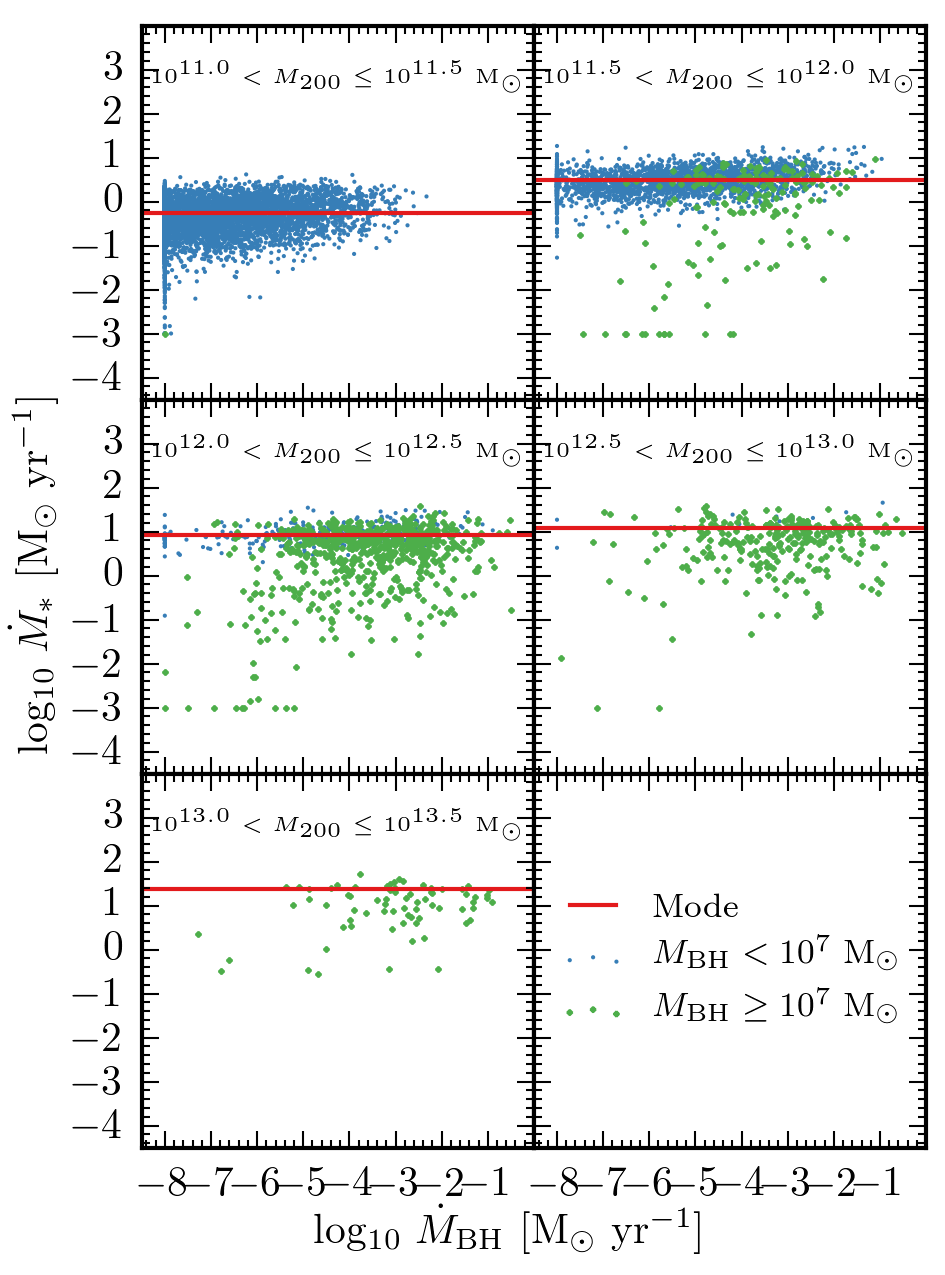
\includegraphics[width=\columnwidth]{plots/SFRvsBHAR_ByHalo}

\caption{Growth rates at $z=1$ (from \cref{fig:sfr_vs_bhar_z1}) for central
galaxies separated into five continuous halo mass ranges. Points are coloured
green if a galaxy hosts a massive BH (\M{BH} $\geq 10^{7}$\Msol) and blue
otherwise. The characteristic SFR for a given halo mass bin (classified as the
mode of the distribution) is shown as a horizontal solid red line. Each range
of halo mass yields a relatively narrow distribution of SFRs ($1-2$~dex) and
much wider distribution of BHARs (up to 8~dex).  Larger halos are associated
with larger characteristic SFRs and have a higher fraction of BHARs $>
10^{-4}$\Msolyr. Galaxies harbouring SFRs far below the characteristic rate all
contain massive BHs (green points) and have likely recently undergone a violent
episode of AGN feedback reducing the current star-forming capability of the
system.}

\label{fig:sfr_vs_bhar_byhalo} \end{figure}

As observational surveys are subject to various flux limitations, they can only
sample particular regions of the full SFR--BHAR plane.  If the global
underlying relation is linear, and each property exhibits a moderate scatter,
each sub sample should also return a linear result.  However, as the findings
of previous sections do not to support an underlying linear relation, and
because the scatter is large, it is important to investigate the effect of this
sampling. 

\cref{fig:sfr_vs_bhar_z1} shows the complete SFR--BHAR plane for all central
galaxies at $z=1$. In order to eliminate any potential bias incurred via
redshift evolution in either growth rate we consider a discrete redshift rather
than the continuous ranges of \cref{sect:observations}. Each data point
represents the \textit{instantaneous} state of a single galaxy and its central
BH, coloured by the halo mass.  Values that are below $10^{-8}$~\Msolyr for
\BHAR and $10^{-3}$~\Msolyr for \SFR are treated as \squotes{zero} and are
clipped to these values. The approximate flux limit of the AGN selected sample
by \citet{Stanley2015} is shown as a solid vertical line and the approximate
flux limit of the SFR selected sample by \citet{Delvecchio2015} is shown as a
horizontal solid line.

It is further apparent that the global relationship between SFR and BHAR is not
simply linear (reference with the dashed green line). Instead, a complicated
relationship arises due to an amalgamation of three distinct behaviours of BH
growth dependent on the mass of the host dark matter halo (see next section).
It is therefore crucial to consider the particular region sampled before
arriving at a particular conclusion.  AGN selected samples, such as that of
\citet{Stanley2015}, currently probe a relatively limited region at the tip of
the SFR--BHAR plane.  With the exception of a few sources with rates \SFR $\ll
1$\Msolyr, galaxies satisfying this selection criteria are distributed over a
relatively narrow range of SFRs. As such, each bin of BHAR yields a very
similar value of \av{SFR}, creating an approximately flat trend.  SFR selected
samples, such as that of \citet{Delvecchio2015}, sample a not too dissimilar
distribution of SFRs (this time due to the flux limit), however, the
distribution of BHARs is much wider.  This in turn yields a steeper relation.
We note, that whilst the mean SFR provides a good proxy of the median SFR for
an AGN selected study (compare columns 3 and 6 of \cref{table:slopes}), the
mean BHAR for a SFR selected study is not a good proxy of the median value due
to the distribution of BHARs having such a large scatter (compare columns 8 and
10 of \cref{table:slopes}).  Although only the results from $z=1$ have been
shown here, when investigated we find the results remain true independent of
redshift.

We therefore conclude that the different behaviour found for the \av{SFR}--BHAR
and \av{BHAR}--SFR relations recovered by observational studies is due to
sampling considerably different regions of the full (not universally linear)
SFR--BHAR plane. We now continue to investigate the nature of this relationship
in the \eagle simulation and its evolution through time.

\subsection{The connection to the host dark matter halo}
\label{sect:to_halo}

The relationship between SFR and BHAR seen in \cref{fig:sfr_vs_bhar_z1} is
complicated, seemingly not adhering to a simple universal trend.  However,
there is evidence that each property has a link with the mass of the host dark
matter halo, highlighted in the change of the data point colours, which
transition smoothly from blue to red with increasing SFR, and systematically
shift rightward in BHAR (with a large scatter) at high halo mass.    

To examine this in more depth we sub categorize the $z=1$ central galaxies into
five continuous ranges of halo mass, showing the growth rates in
\cref{fig:sfr_vs_bhar_byhalo}.  Here we find, in fact, that the global make up
of the SFR--BHAR plane in \cref{fig:sfr_vs_bhar_z1} is resolved into a
collection of two dimensional strips, wide in their dynamic range of BHAR
($\approx 4-6$~dex) yet generally much more compact in their SFR ($\approx
1-2$~dex).  Each strip hosts a characteristic value of SFR (defined as the mode
of the distribution, shown as a horizontal solid red line) that continuously
increases with increasing halo mass. This is in line with the \squotes{star
forming main sequence}, where galaxies of increased stellar mass are seen to
host larger SFRs \citep[e.g,][]{Elbaz2007}. Interestingly, the rate of change
with \M{200} for this characteristic SFR does not remain constant, initially
increasing by $\Delta$\SFR $\approx 1$ dex between $10^{11.0} <$ \M{200} $ \leq
10^{12.0}$\Msol and reducing to almost zero in the regime $10^{12.5} < $
\M{200} $ \leq 10^{13.5}$\Msol. This is potential evidence that SFRs in massive
systems are not keeping pace with the increasing baryonic inflow rates for
increasing halo mass at fixed redshift \citep[e.g,][]{Correa2015}. BHARs show a
less continuous behaviour however, broadly categorized by two rudimentary
states: BHs residing in haloes below $\approx 10^{11.5}$\Msol are typically
accreting at a \squotes{low} rate (\BHAR $\ll 10^{-4}$~\Msolyr); BHs residing
in haloes more massive than $\approx 10^{12.5}$\Msol tend to be accreting at a
\squotes{high} rate (\BHAR $> 10^{-4}$~\Msolyr). The fraction of galaxies with
\BHAR $\geq 10^{-4}$\Msolyr for a given halo mass bin is $\approx$ 3\%, 21\%,
55\%, 70\% and 78\% from $10^{11.0} <$ \M{200} $\leq 10^{11.5}$\Msol to
$10^{13.0} <$ \M{200} $\leq 10^{13.5}$\Msol respectively.  Those in haloes
between the mass range $10^{11.5} \sim 10^{12.5}$\Msol are in an intermediate
state. 

A fraction of galaxies hosted by haloes with \M{200} $\gtrsim 10^{11.5}$\Msol
harbour extremely low, or even zero SFRs. As all of these galaxies host massive
BHs (\M{BH} $\geq 10^{7}$\Msol, green dots), we are most likely seeing the
effect of recent episodes of violent AGN feedback that have severely reduced
the current star-forming capabilities of these systems.  The cause, prevalence
and impact of these feedback events will be the subject of a future paper.

\begin{figure}
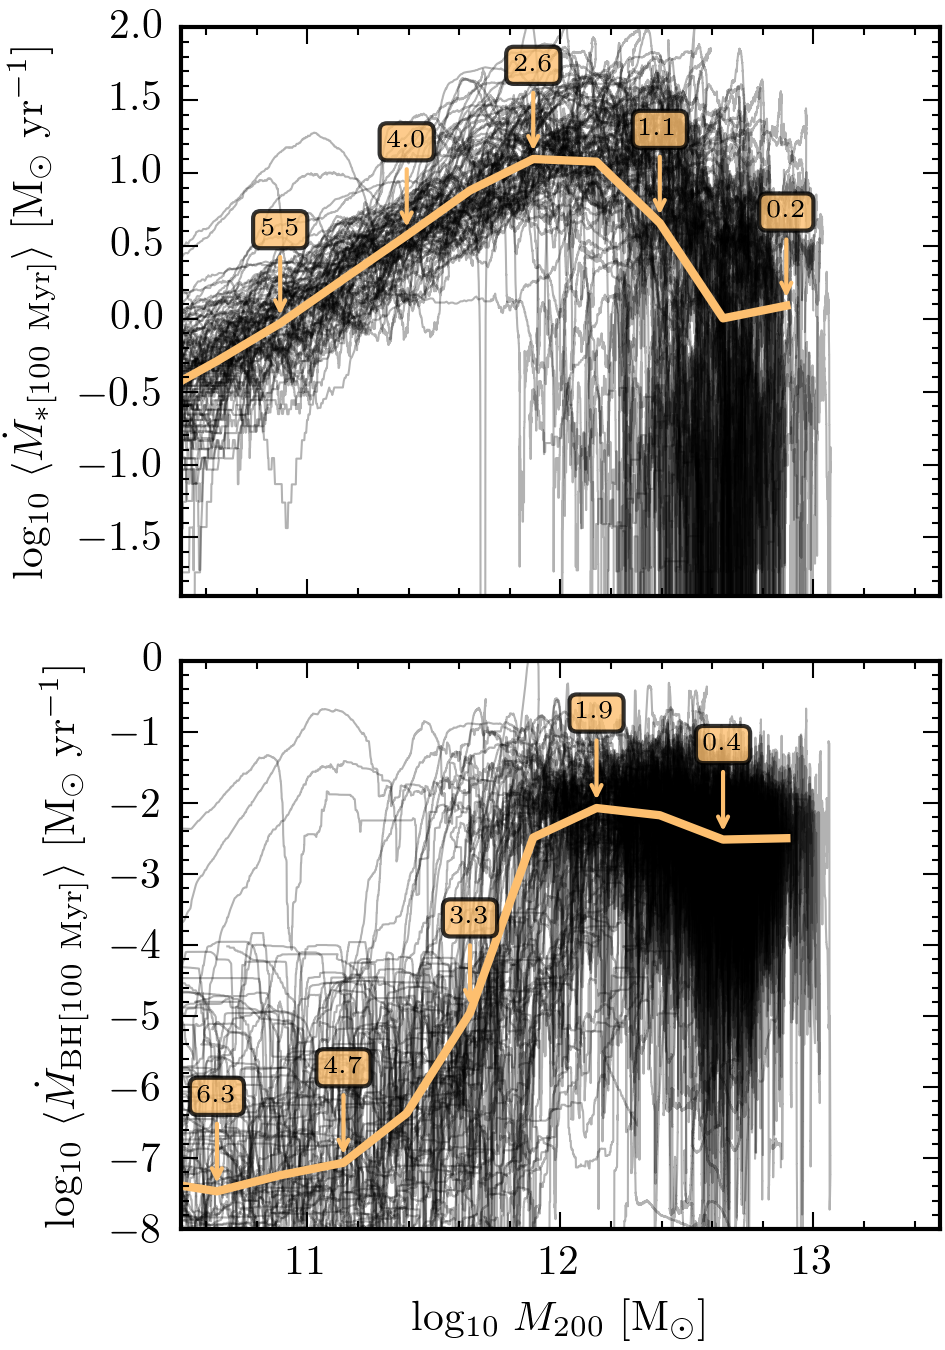
\includegraphics[width=\columnwidth]{plots/OneSquare}

\caption{The evolutionary history of SFR (top panel) and BHAR (bottom panel) as
a function of halo mass for all galaxies that come to reside in the $10^{12.5}
< M_{\mathrm{200}} < 10^{13.0}$\Msol, $10^{8.0} < M_{\mathrm{BH}} <
10^{8.5}$\Msol two-dimensional bin of \cref{fig:bhm_vs_hm} at $z=0$ (outlined
in yellow). Each black line is an individual history. The orange line shows the
median trend, annotated with the median redshift at which these galaxies were
hosted in haloes of that mass.  For each panel, growth rates are time-averaged
over 100~Myr as to overcome the noise induced when considering instantaneous
rates.  We see very different evolutionary behaviour for SFR and BHAR as the
halo grows. SFRs initially rise and then decline, centred around \M{200} $\sim
10^{12}$\Msol. BHARs similarly transition from a low to high rate around this
halo mass.}

\label{fig:one_square} \end{figure}

\begin{figure}
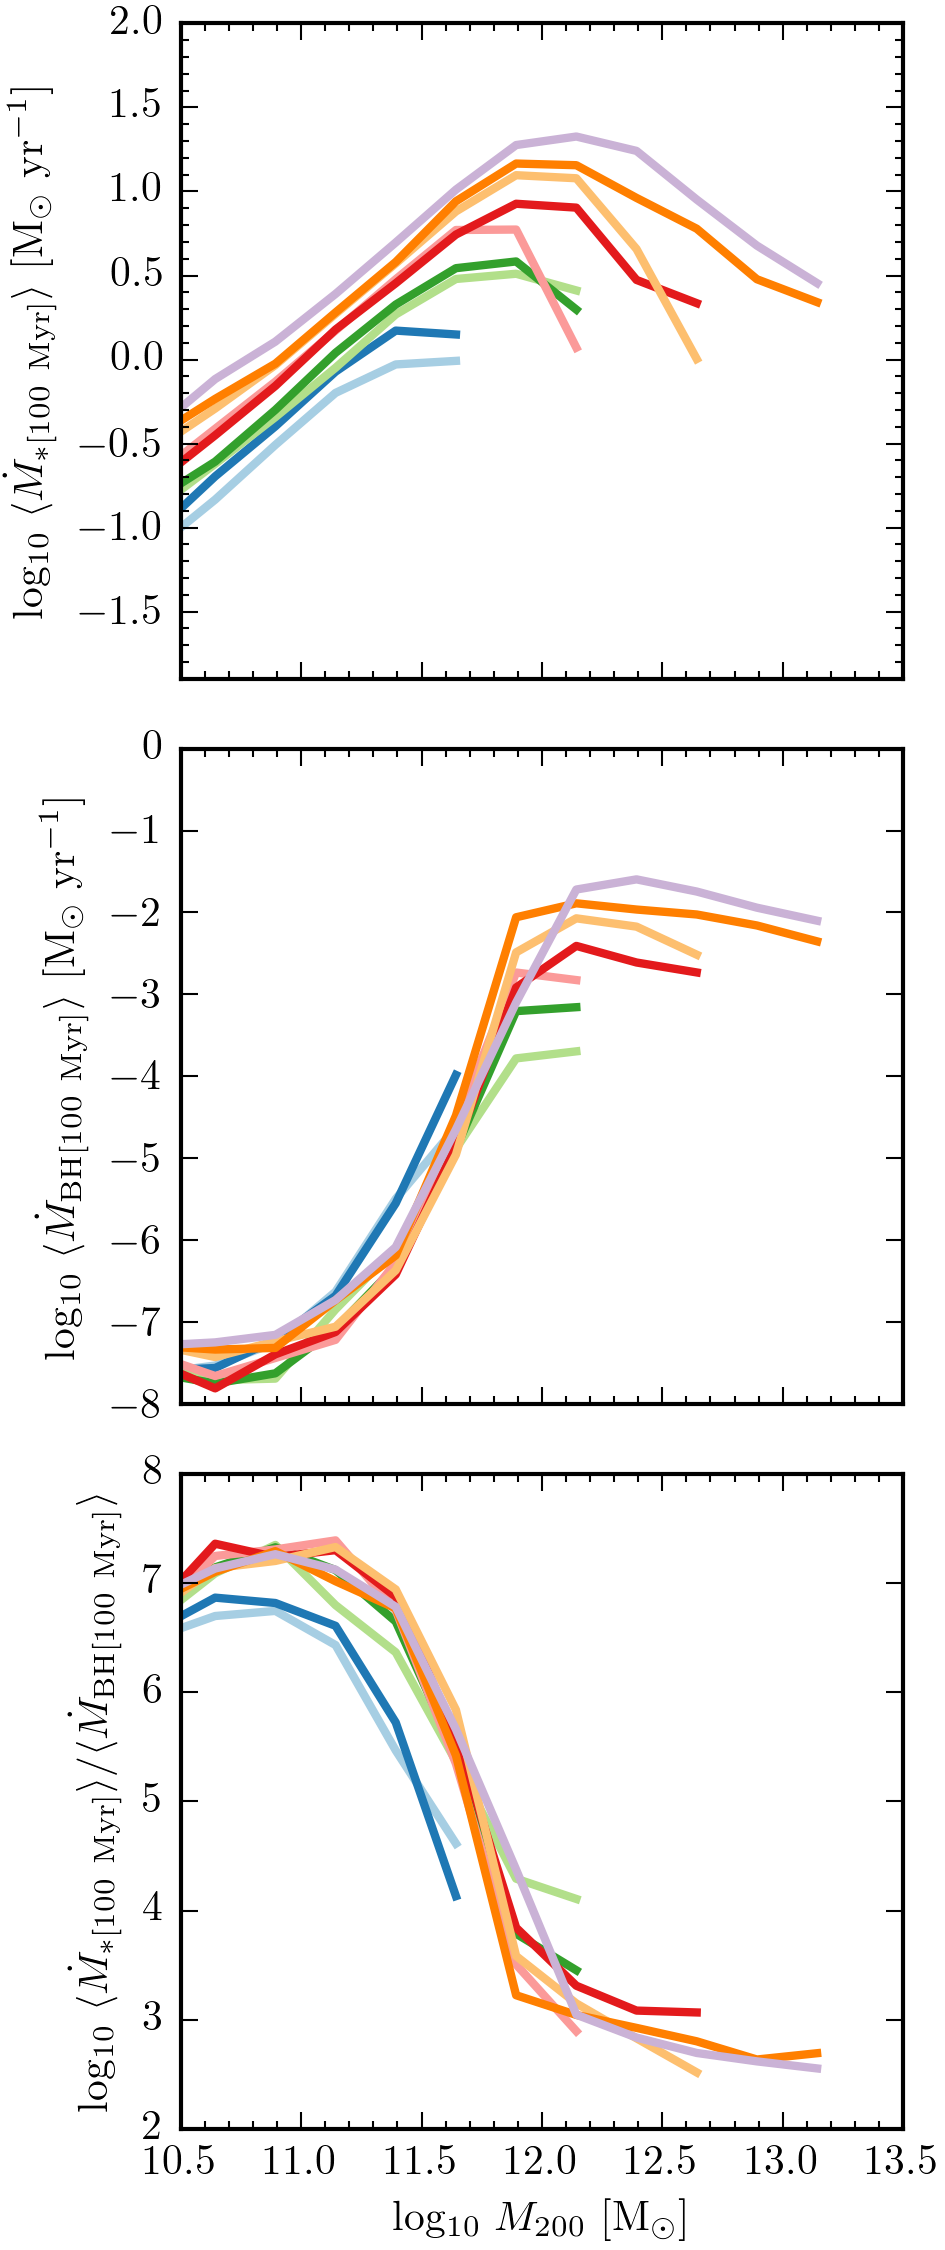
\includegraphics[width=\columnwidth]{plots/AllSquares}

\caption{\textit{top two panels}: A continuation of the analysis in
\cref{fig:one_square} to each of the nine chosen two-dimensional bins of
\cref{fig:bhm_vs_hm}. The lines are the median track, with the colour
corresponding to the outline in \cref{fig:bhm_vs_hm}. Regardless of where a
galaxy is located on the \M{BH}--\M{200} plane at the present day, both the
galaxy and its central BH evolve similarly, though different from each other.
The change in normalisations between the histories is due to the declining
baryonic inflow rates with decreasing redshift for a fixed halo mass.
\textit{bottom panel}: The median ratio between the SFR and BHAR from the two
panels above. SFRs are initially dominant by many orders of magnitude in low
mass haloes (\M{200} $\lesssim 10^{11.5}$\Msol), coming to plateau at an
approximately constant value of $\sim 10^{3}$ in high mass haloes (\M{200}
$\gtrsim 10^{12.5}$\Msol).}

\label{fig:avHistory_vs_hm}
\end{figure}

We now investigate if the growth rate to halo connection evolves.  To do this
we return to the \M{BH}--\M{200} relation shown for $z=0$ in
\cref{fig:bhm_vs_hm}. The population is sub divided into two-dimensional bins,
0.5~dex on a side and outlined as squares.  Here we investigate nine bins that
lie along the median track through a continuous range spanning $10^{11.5} <$
\M{200} $< 10^{13.5}$\Msol in halo mass and $10^{6.0} <$ \M{BH} $<
10^{9.0}$\Msol in BH mass, each outlined with a unique colour to reference
their histories in
\cref{fig:one_square,fig:avHistory_vs_hm,fig:sfr_vs_bhar_av}.

\cref{fig:one_square} shows the evolution of the time-averaged SFR (top panel)
and time-averaged BHAR (bottom panel) as a function of halo mass for all
galaxies that come to reside in one of these two-dimensional bins at the
present day (each solid black line is an individual history). We time-average
both SFR and BHAR over 100~Myr in order to remove the inherent noise when
considering instantaneous growth rates, and unveil the average trend.  To
eliminate galaxies that were previously classified as satellites of a more
massive halo, we only consider central galaxies that have evolved monotonically
in their halo mass (this excludes only $\approx 1\%$ of the $z=0$ centrals
population).  We see, that although individual histories can be quite
different, on average galaxies and their central BHs do follow a well defined
path.  The median SFR and BHAR of this population subset for a given halo mass
are over-plotted in yellow, annotated by the median redshift at which they were
hosted by haloes of that particular mass.  As expected, an increasing halo mass
corresponds to a decreasing redshift.

There is a striking difference in behaviour seen between the two growth rates
as the halo grows.  Initially the SFR increases steadily with halo mass. As the
halo grows more massive than $\approx 10^{12}$\Msol the SFRs begin to fluctuate
between high and low values, yet overall there is a gradual decline of the
median trend after this mass.  Similarly, BHARs also change their behaviour
around $\approx 10^{12}$\Msol, rapidly transitioning from a low (\BHAR $\ll
10^{-4}$\Msolyr) to high (\BHAR $> 10^{-4}$\Msolyr) rate. As with SFRs, BHARs
decline a similar amount after the halo mass $\approx 10^{12}$\Msol (note the
many orders of magnitude difference in the scale of the growth rate axis
between the two panels).  We interpret therefore, given that the decline of SFR
coincides with the peak of the rapid increase in BHAR, that AGN feedback is
impeding the continued rise of SFRs in the most massive systems (see
\cref{fig:variability} for an individual example of SFR reduction after the
peak AGN activity at lookback time $\approx 12$).  We note that the decrease in
halo mass accretion rate with declining redshift and the dependence of halo
cooling rates on halo mass will play \textit{additional} roles in shaping these
histories. However, given the severity of the SFR reduction seen immediately
after the BHAR peak, AGN feedback appears to be a dominant factor in hindering
further galaxy growth.

\cref{fig:avHistory_vs_hm} extends this analysis to each of the highlighted
two-dimensional bins in \cref{fig:bhm_vs_hm}, now showing only the median lines
for clarity. Remarkably, the evolutionary behaviour is similar regardless of
the final position in the \M{BH}--\M{200} plane.  The normalisation of each
history is set by the evolving baryonic inflow rate at fixed halo mass. As this
rate decreases with redshift \citep[e.g,][]{Correa2015}, so does the
normalisation of both the SFR and BHAR seen here (as each population reaches a
particular halo mass at different times). We include also in the bottom panel
of \cref{fig:avHistory_vs_hm} the median ratio between SFR and BHAR shown in
the two panels above. This shows that galaxy growth is dominant over BH growth
by many orders of magnitude in low mass haloes (\M{200} $\lesssim
10^{11.5}$\Msol). As BHARs settle to their \squotes{high} rate in haloes of a
mass above \M{200} $\sim 10^{12}$, the ratio between SFR and BHAR plateaus to
an approximately constant value of $\sim 10^{3}$.  Note the trends of both
\cref{fig:one_square,fig:avHistory_vs_hm} are not directly observable as they
rely on median time-averaged growth rates in both SFR and BHAR of 100~Myr
whilst also being binned by halo mass. 
